\documentclass[8pt]{beamer}
\usepackage[utf8]{inputenc}
\usetheme{default}
\fontfamily{ppl}

\usetheme{Antibes}
\usecolortheme{spruce}

\usefonttheme{serif} 

\title{APC Project: SimpleQuadTree}
\author{Thomas Bellotti}
\date{\today}

%\usepackage{mathpazo} % add possibly `sc` and `osf` options


\begin{document}

\begin{frame}
 \maketitle
\end{frame}


\section{Introduction}
\begin{frame}
 \begin{center}
  \begin{huge}
   Introduction
  \end{huge}
 \end{center}
\end{frame}

\subsection{Aims of the project}
\begin{frame}
\frametitle{Aims of the project}
\pause
Original target:
\begin{block}{Aim 1}
 Construct \textbf{highly adaptive Cartesian non-uniform meshes} on which we can perform \textbf{numerical quadrature} and eventually implement \textbf{numerical solvers for PDEs}, mainly based on the Finite Volume method.
\end{block}
\pause
After some work...
\begin{block}{Aim 2}
Implement a simple method to \textbf{compress digital images}, which recognizes large areas of almost uniform color. Could be eventually used also for shape recognition. 
\end{block}
\pause

These two objectives may seems quite far one from the other but actually they can be linked by... \textbf{Quadtrees}.

\end{frame}
\begin{frame}

\subsection{Quadtrees}
\frametitle{What is a quadtree}
\pause
Basically just an unbalanced tree structure allowing \textbf{four children}. Generalized in 3D by the octrees.
 \pause
 It has a clear geometrical counterpart in terms of AMR (Adaptive Mesh Refinement), where they are built by \textbf{recursively splitting} larger cells.
\begin{figure}[!h]
\begin{center}
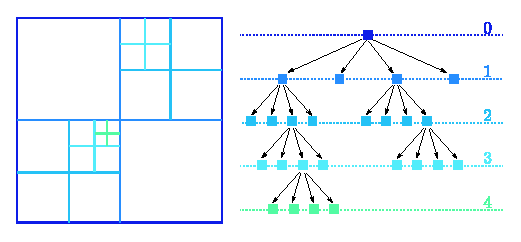
\includegraphics[width=0.8\textwidth]{./figures/quadtree.eps}

\begin{tiny}
Image from: T. Bellotti, M. Theillard - A coupled level-set and reference map method for interface representation with applications to two-phase flows simulation - 2018 in press: J. Comput. Phys.
\end{tiny}
\end{center}
\end{figure}
\end{frame}
\subsection{Some terminology}
\begin{frame}
 \frametitle{Some terminology}
 \pause
 \begin{itemize}
 \item \textbf{Leaf}: cell without children.\pause
  \item \textbf{Level} (of a cell): number of times the largest cell has been split to generate the current cell.\pause
  \item \textbf{Maximum level} ($\text{max}_{\text{level}}$): maximum number of allowed splits.
  \item \textbf{Minimum level} ($\text{min}_{\text{level}}$): minimum number of necessary splits.
 \end{itemize}

\end{frame}

\section{Models and tools to understand what follows}
\begin{frame}
 \begin{center}
  \begin{huge}
   Models and tools to understand what follows
  \end{huge}
 \end{center}
\end{frame}
\subsection{Level-set theory}
\begin{frame}
 \frametitle{Level-set theory}
 \pause
 In this work, we only see it as a \textbf{strategy to build} beautiful and meaningful \textbf{adaptive meshes} (there is more than this).\pause
 \begin{figure}[!h]
\begin{center}
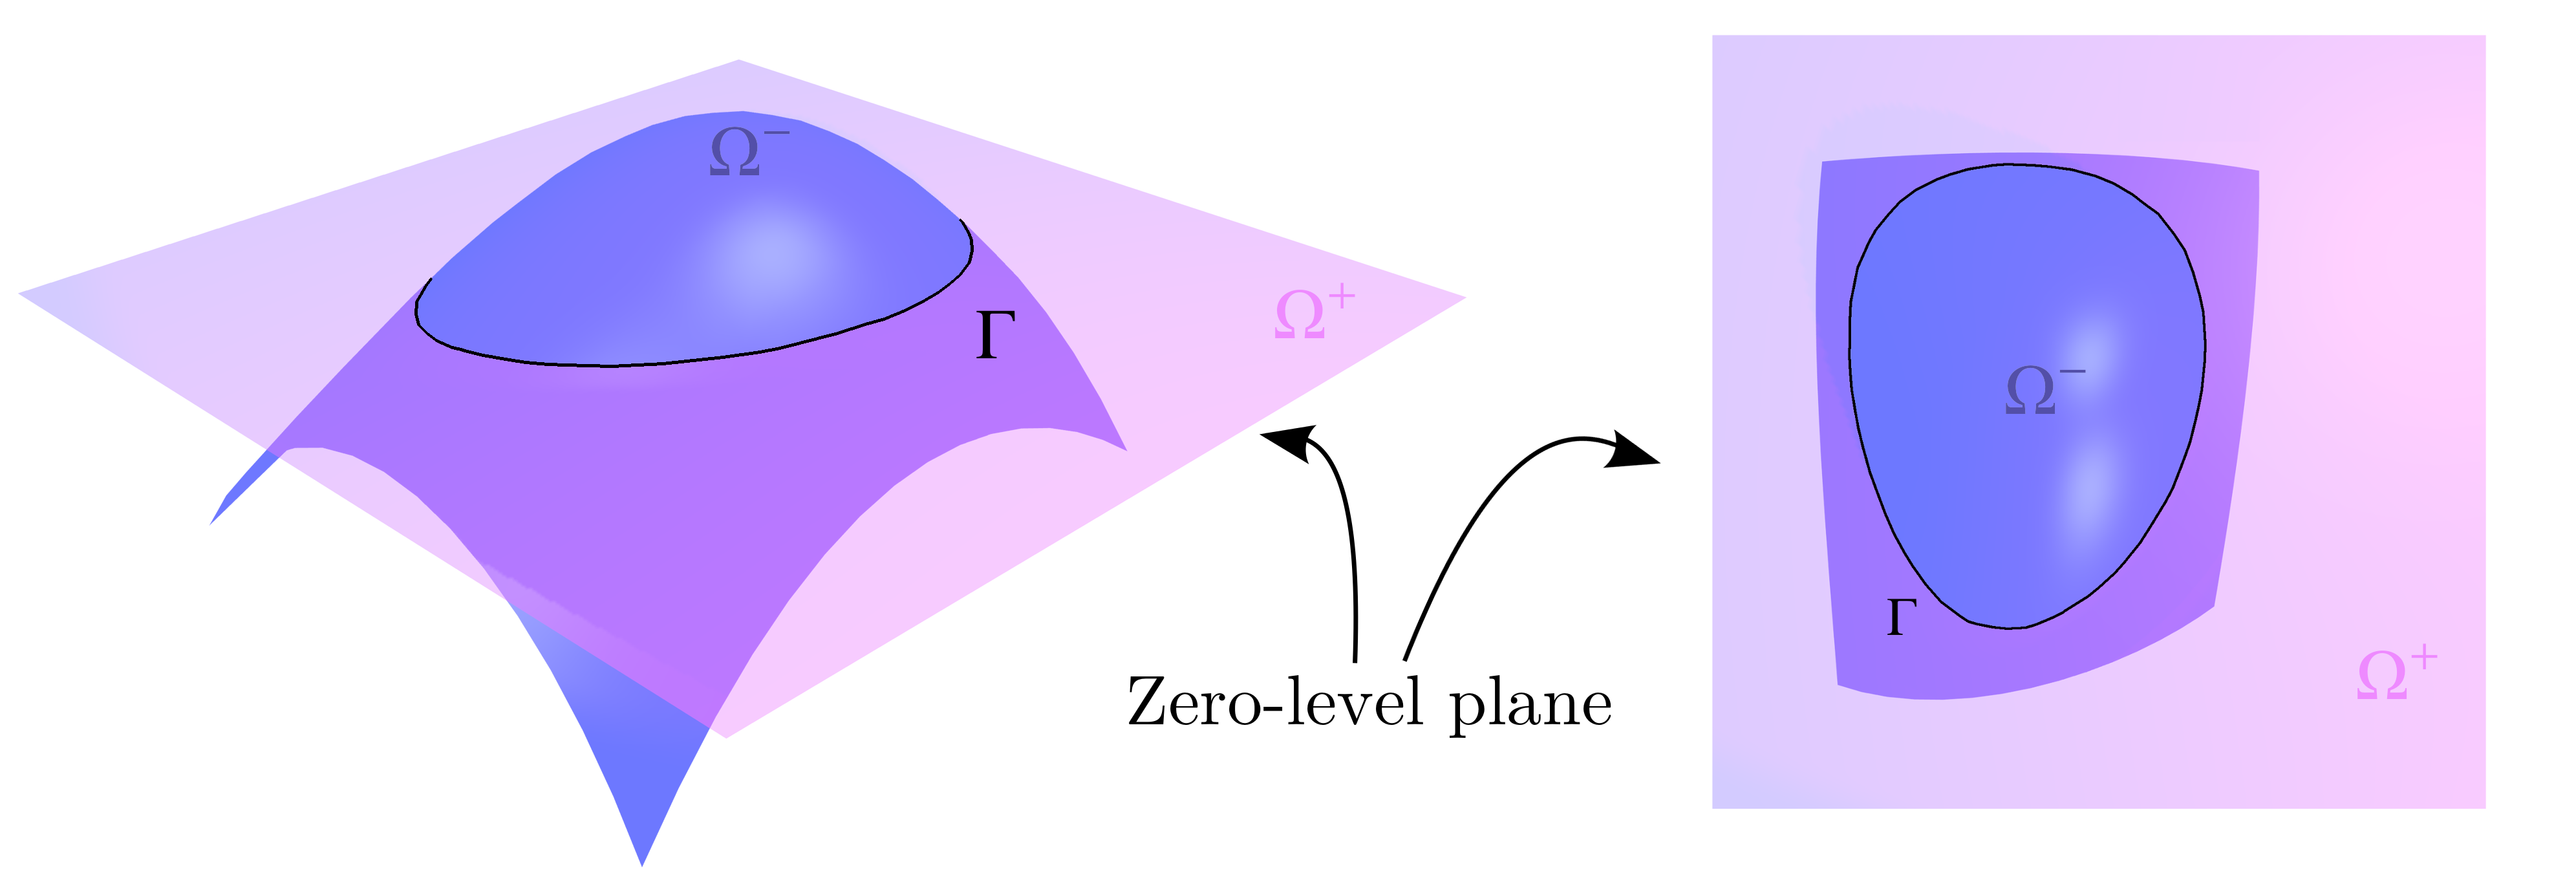
\includegraphics[width=0.7\textwidth]{./figures/levelset}

\begin{tiny}
Image from: T. Bellotti, M. Theillard - A coupled level-set and reference map method for interface representation with applications to two-phase flows simulation - 2018 in press: J. Comput. Phys.
\end{tiny}
\end{center}
\end{figure}
\begin{flalign*}
\Gamma &= \left \{ \mathbf{x} \in \Omega ~ : ~ \phi(\mathbf{x}) = 0 \right \}, \nonumber \\
\Omega^- &= \left \{ \mathbf{x} \in \Omega ~ : ~ \phi(\mathbf{x}) < 0 \right \}, \label{eq:levelsetdef} \\
\Omega^+ &= \left \{ \mathbf{x} \in \Omega ~ : ~ \phi(\mathbf{x}) > 0 \right \}.\nonumber 
\end{flalign*}
\end{frame}

\begin{frame}
  \frametitle{Level-set theory}
It is probably the easiest way of \textbf{representing an interface} in a computationally efficient manner.
\pause
\begin{block}{Example}
 In 2D, a circle centered in $(x_0, y_0)$ with radius $R$ can be represented by:
 \begin{equation*}
  \phi(x,y) = \sqrt{(x-x_0)^2 + (y-y_0)^2} - R.
 \end{equation*}
 \pause
\end{block}
Notice that, given $\Gamma$, the level-set is not unique, but this is not our problem now. It is unique if we assume (and we will do so) that $\phi(x,y)$ is nothing but the \textbf{signed distance} of $(x,y)$ from $\Gamma$.
\pause
\begin{equation*}
 \text{split ~}\mathcal{C} ~ \text{if} \quad : \quad  \left | \phi(\mathbf{x}_{\mathcal{C}}) \right | \leq \text{Lip}(\phi) \cdot \text{diag}(\mathcal{C}) \qquad \text{and} \qquad \text{level}(\mathcal{C}) \leq \textrm{max}_{\textrm{level}},
\end{equation*}
This naively means that we split a cell wheather its diagonal length exceeds the distance from the interface $\Gamma$ represented by the level-set $\phi$.
\end{frame}

\begin{frame}
 And the result can be\dots Very nice!
  \begin{figure}[!h]
\begin{center}
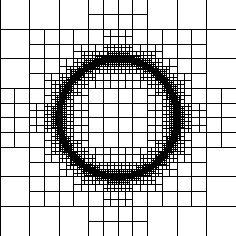
\includegraphics[width=0.5\textwidth]{./figures/integrator/pi_1.pdf}
\end{center}
\end{figure}
 
\end{frame}



\subsection{Gaussian quadrature}
\begin{frame}
 \frametitle{Gaussian quadrature}
 \pause
 Considering a stardard quadrilateral domain $\Omega = [-1,1]^2$ and given a possibly smooth function $f : \Omega \to \mathbb{R}$, we want to compute:
 \begin{equation*}
  \int_{\Omega} f(x,y)dxdy.
 \end{equation*}
This can be done by quadrature formulae, based on simple evaluation of the function $f$ at certain points of the domain.
For our purpose, we use two choices:\pause
\begin{enumerate}
 \item \textbf{``Naive'' formula}, with only one function evaluation.
 \begin{equation*}
  \int_{\Omega}f(x,y)dx dy \simeq |\Omega| f(0,0)  = 4 f(0,0)
 \end{equation*}\pause
 \item \textbf{3rd order Gaussian formula}, with nine function evaluations (plus extra computations to adapt to a generic domain).
 \begin{align*}
  \int_{\Omega} f(x,y)dx dy &\simeq \frac{5}{81} \left [ 5 f \left (-\sqrt{\frac{3}{5}},-\sqrt{\frac{3}{5}} \right ) + 8 f \left (0,-\sqrt{\frac{3}{5}} \right ) + 5 f \left (\sqrt{\frac{3}{5}},-\sqrt{\frac{3}{5}} \right )\right ] \\
  &+\frac{8}{81} \left [ 5 f \left (-\sqrt{\frac{3}{5}},0 \right ) + 8 f \left (0,0 \right ) + 5 f \left (0,\sqrt{\frac{3}{5}} \right )\right ] \\
  &+\frac{5}{81} \left [ 5 f \left (-\sqrt{\frac{3}{5}},\sqrt{\frac{3}{5}} \right ) + 8 f \left (0,\sqrt{\frac{3}{5}} \right ) + 5 f \left (\sqrt{\frac{3}{5}},\sqrt{\frac{3}{5}} \right )\right ].
 \end{align*}

\end{enumerate}

\end{frame}


\subsection{Rgb colors and their ``distance''}
\begin{frame}
 \frametitle{Rgb colors and their ``distance''}
 \pause
 It is probably the simplest way of representing colors, as a combination of three components, \textbf{\textcolor{red}{red}, \textcolor{green}{green} and \textcolor{blue}{blue}}.
 Thus, a color $C$ is nothing else than a triplet:
 \begin{equation*}
  C = \left [ \textcolor{red}{C_{\text{red}}}, \textcolor{green}{C_{\text{green}}}, \textcolor{blue}{C_{\text{blue}}} \right ],
 \end{equation*}
where $\textcolor{red}{C_{\text{red}}},\textcolor{green}{C_{\text{green}}},\textcolor{blue}{C_{\text{blue}}} \in \{0,\dots, 255 \}$. In this way, we can represent 16,777,216 different tones.
 \pause
 For our purpose, it is useful to define the notion of \textbf{distance} between two colors, which can be defined in many ways. In our case, we use the simple ``corrected'' formula:
 \begin{equation*}
  d(C^1,C^2) = \sqrt{\textcolor{red}{2 \left (C^1_{\text{red}}-C^2_{\text{red}} \right )^2} + \textcolor{green}{4 \left (C^1_{\text{green}}-C^2_{\text{green}} \right )^2} + \textcolor{blue}{3 \left (C^1_{\text{blue}}-C^2_{\text{blue}} \right )^2}}.
 \end{equation*}\pause
The mean color between $\left \{ C^1, \dots, C^N\right \} $ is defined by:
\begin{equation*}
 \overline{C} \left ( \left \{ C^1, \dots, C^N\right \} \right ) = \left[ \textcolor{red}{\frac{1}{N} \sum_{n=1}^N C_{\text{red}}^n}, \textcolor{green}{\frac{1}{N} \sum_{n=1}^N C_{\text{green}}^n},\textcolor{blue}{ \frac{1}{N} \sum_{n=1}^N C_{\text{blue}}^n}\right ],
\end{equation*}\pause
and a sort of standard deviation as:
\begin{equation*}
 \sigma  \left ( \left \{ C^1, \dots, C^N\right \} \right ) = \frac{1}{N} \sqrt{\sum_{n=1}^N d(C_n,\overline{C})^2} \in [0,765].
\end{equation*}
\end{frame}

\begin{frame}
 \frametitle{How to compress an image?}
 \pause
 Let $\mathcal{P}$ be a preleave whose children are $\mathcal{L}(\mathcal{P})$. We define a tolerance $0< \epsilon \ll 1$. Then:
 \begin{equation*}
  \text{merge} \quad \mathcal{P} \quad \text{if} ~ : ~ \sigma  \left ( \mathcal{L}(\mathcal{P}) \right ) \leq 765 \cdot \epsilon.
 \end{equation*}\pause
In the case of merging, we consider:
\begin{equation*}
 C_{\mathcal{P}} = \overline{C} \left ( \mathcal{L}(\mathcal{P}) \right ).
\end{equation*}

\end{frame}



\section{Implementation}
\begin{frame}
 \begin{center}
  \begin{huge}
   Implementation
  \end{huge}
 \end{center}
\end{frame}


\subsection{Classes}
\begin{frame}
 \frametitle{The Cell class}
 \pause
  \begin{figure}[!h]
\begin{center}
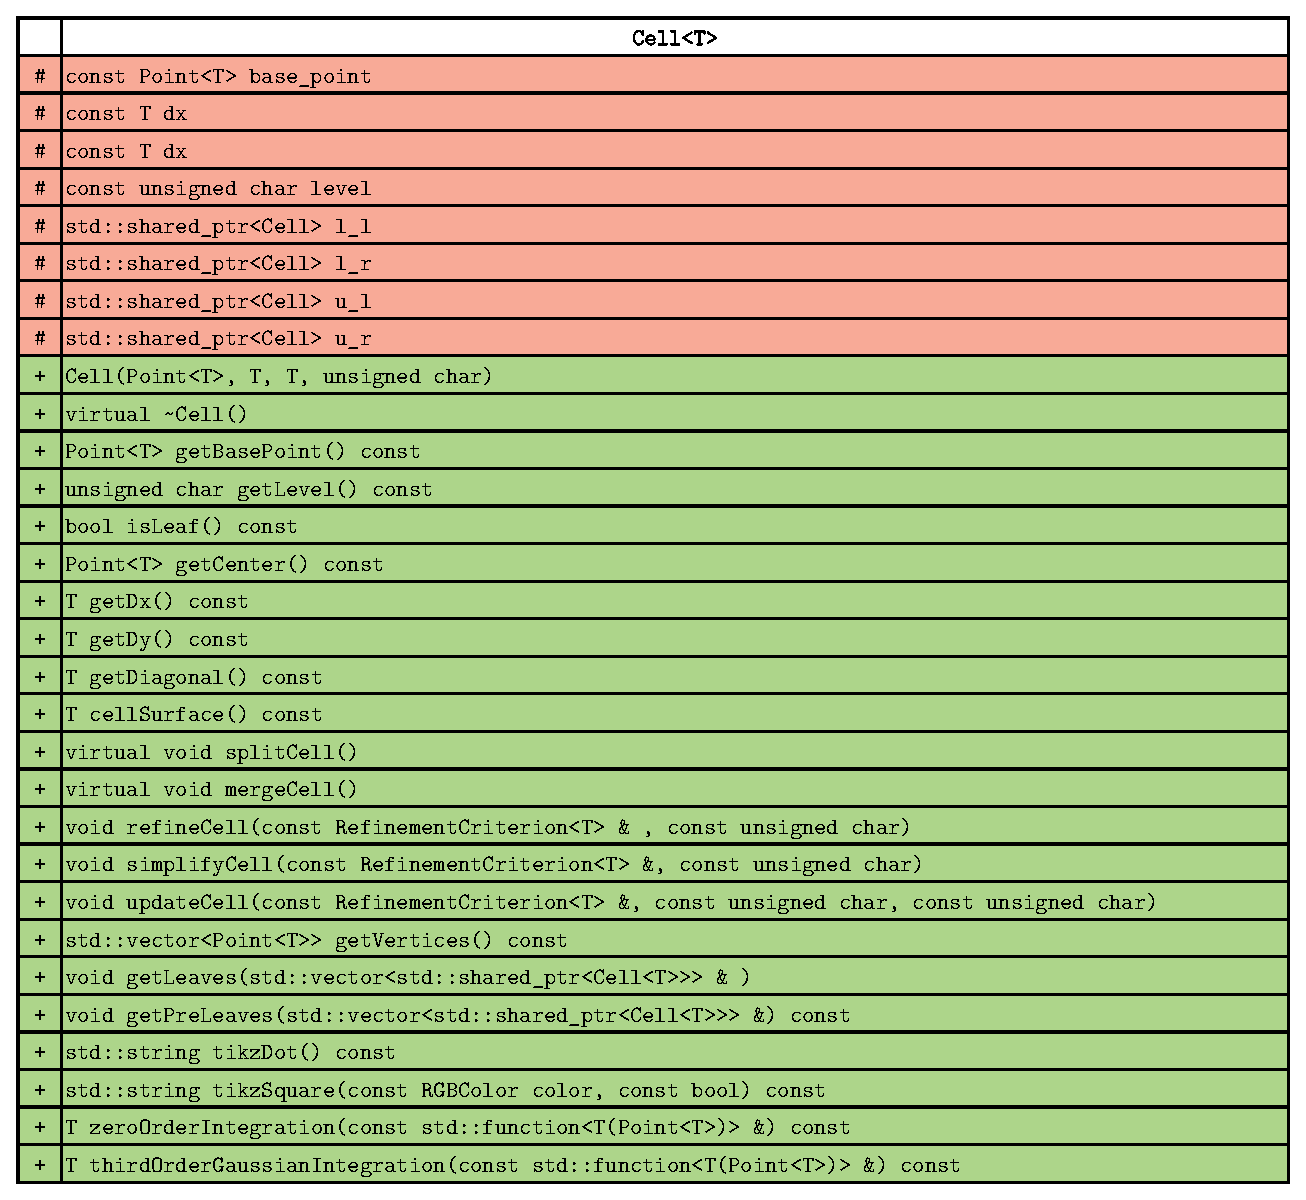
\includegraphics[width=0.75\textwidth]{./figures/cell_h.eps}
\end{center}
\end{figure}
\end{frame}

\begin{frame}
 \frametitle{The Pixel class inheriting from Cell}\pause
 The ``generalized'' pixel is basically a Cell...
  \begin{figure}[!h]
\begin{center}
\includegraphics[width=0.6\textwidth]{./figures/pixel_h.eps}
\end{center}
\end{figure}
plus a \textbf{color}.
We have to be careful to \textbf{cast pointers} when we need to extract information from the Pixel.
\end{frame}

\begin{frame}
 \frametitle{The QuadTree class}\pause
This class is mostly a \textbf{wrapper} of the Cell class, but it is what the user interacts with.
\begin{figure}[!h]
\begin{center}
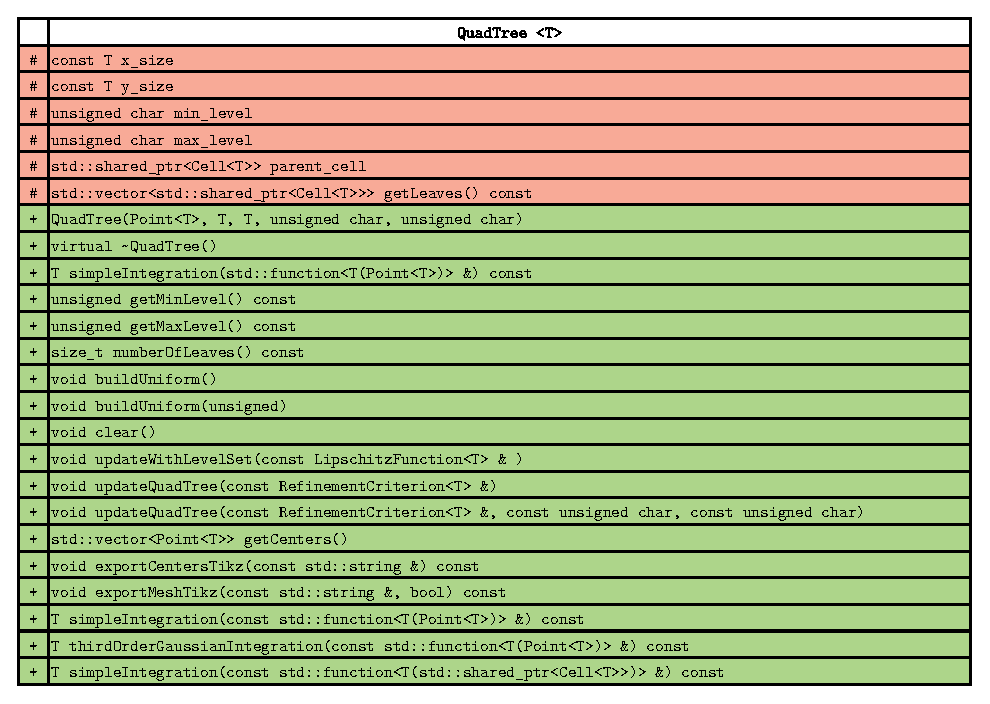
\includegraphics[width=0.9\textwidth]{./figures/quadtree_h.eps}
\end{center}
\end{figure}
\end{frame}

\begin{frame}
 \frametitle{The Image class}\pause
This class is mostly a \textbf{wrapper} of the Pixel class.
We distinguished it from the QuadTree class (it does not inherit from it) because there are many features that they do not share.
\begin{figure}[!h]
\begin{center}
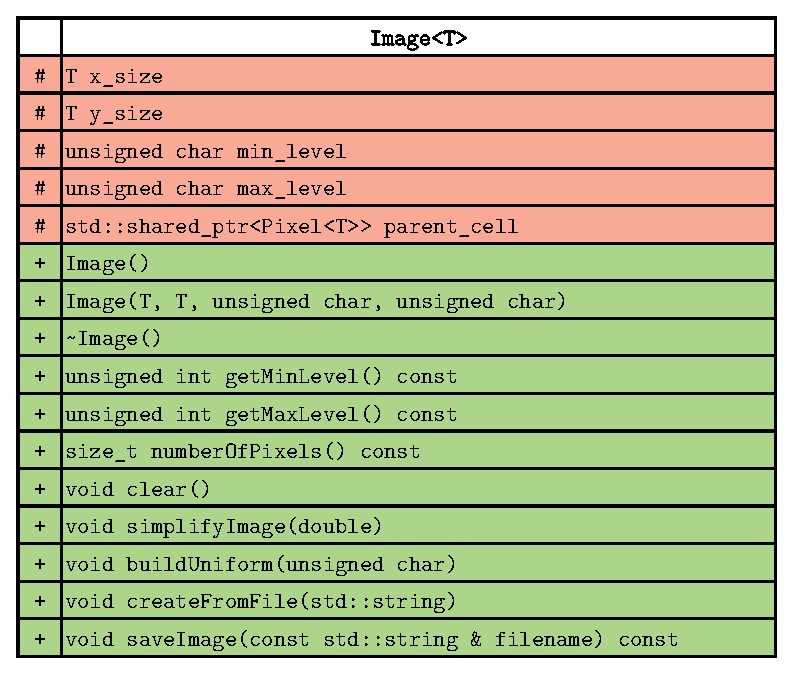
\includegraphics[width=0.5\textwidth]{./figures/image_h.eps}
\end{center}
\end{figure}
\end{frame}

\begin{frame}
 \frametitle{The way we update the mesh: the RefinementCriterion class}\pause
This is a very simple \textbf{abstract class} with an operator telling us if we have to split a Cell or not.
\begin{figure}[!h]
\begin{center}
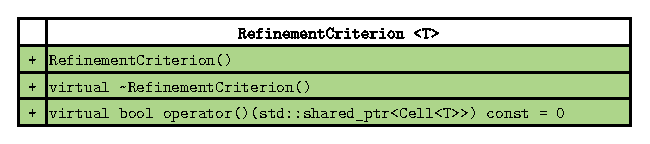
\includegraphics[width=0.6\textwidth]{./figures/refinementcriterion_h.eps}
\end{center}
\end{figure}\pause
Many important criteria inherit from it:
\begin{figure}[!h]
\begin{center}
\includegraphics[width=0.6\textwidth]{./figures/RefineAlwaysCriterion_h.eps}
\includegraphics[width=0.6\textwidth]{./figures/LevelSetCriterion_h.eps}
\includegraphics[width=0.6\textwidth]{./figures/CriterionVariance_h.eps}
\end{center}
\end{figure}
\end{frame}


\subsection{Parallelization of the quadrature}
\begin{frame}
\frametitle{How we parallelize the quadrature}\pause
We want to take advantage of the \textbf{modular nature} of the quadtree structure in order to \textbf{avoid communications} between processes.
\pause

The key idea is to have a number of core which is a power of 4 and have a minimum level large enough, so that we can avoid communications between cores and each of them has a local tree (no shared memory).
 \begin{figure}[!h]
\begin{center}
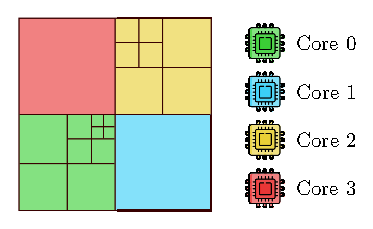
\includegraphics[width=0.65\textwidth]{./figures/parallel_integration.eps}
\end{center}
\end{figure}

And each subtree (core) integrates independently. At the very end, the sub-integrals are summed with a \textbf{reduce} procedure.
\end{frame}

\section{Tests and results}
\begin{frame}
 \begin{center}
  \begin{huge}
   Tests and results
  \end{huge}
 \end{center}
\end{frame}

\subsection{Construction of highly adaptive grids}

\begin{frame}
\frametitle{We are able to construct very general meshes}\pause
 \begin{figure}[!h]
\begin{center}
\includegraphics[width=0.35\textwidth]{./figures/level_set_color.pdf}
\includegraphics[width=0.52\textwidth]{./figures/mandelbrot_criterion_color.pdf} \\
\includegraphics[angle=90, width=0.6\textwidth]{./figures/space_criterion_color.pdf}
\end{center}
\end{figure}
\end{frame}

\subsection{Numerical quadrature}

\begin{frame}
\frametitle{We are able to perform parallel quadratures}
\textbf{FINO A QUA!}
Computations have been tested on \textbf{4 cores} with the following specifications:
\begin{itemize}
 \item Product: Intel(R) Xeon(R) CPU E5-2673 v4 @ 2.30GHz
\end{itemize}
Taking:
\begin{equation*}
 \text{min}_{\text{level}} = 3 \qquad \text{max}_{\text{level}} = 11,
\end{equation*}
so, for the uniform mesh, we deal with
\begin{equation*}
 2^{11} \times 2^{11} \quad \text{cells} = 4'194'304 \quad \text{cells}.
\end{equation*}
Each time, we perform two tests and take the average time in order to avoid spurious effects.
\end{frame}


\begin{frame}\begin{footnotesize}
\begin{gather*}
  \Omega = [-2,2]^2 \quad \phi(x,y) = \sqrt{x^2+y^2}-1 \quad f(x,y) = \mathbb{I}_{\{\phi(x,y) \leq 0\}} \quad
  \int_{\Omega} f(x,y) dx dy = \pi.
\end{gather*}\end{footnotesize}
 \begin{figure}[!h]
\begin{center}
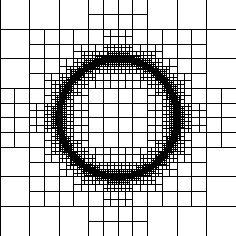
\includegraphics[width=0.32\textwidth]{./figures/integrator/pi_1.pdf}
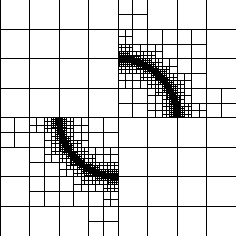
\includegraphics[width=0.32\textwidth]{./figures/integrator/pi_2.pdf}
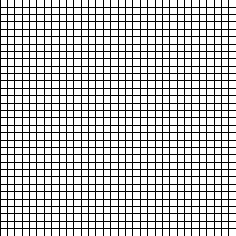
\includegraphics[width=0.32\textwidth]{./figures/integrator/pi_3.pdf}
\end{center}
\end{figure}
\begin{footnotesize}
\begin{center}
\begin{tabular}{|c|c|c|c|c|c|c|c|c|} 
   \hline
    \textbf{Naive} & \multicolumn{2}{|c|}{Mesh 1} & \multicolumn{2}{|c|}{Mesh 2} & \multicolumn{2}{|c|}{Mesh 3}\\
    \hline
    \# of cores & Time [s] & Speedup & Time[s] & Speedup & Time [s] & Speedup \\
    \hline
    1 & 6.585 & - & 6.639 & - & 7.279 & - \\
    4 & 1.721 & \textbf{3.826} & 1.774 & \textbf{3.742} & 1.912 & \textbf{3.807} \\
    \hline
\end{tabular}
\end{center}
\begin{center}
\begin{tabular}{|c|c|c|c|c|c|c|c|c|} 
   \hline
    \textbf{3rd Gaussian}& \multicolumn{2}{|c|}{Mesh 1} & \multicolumn{2}{|c|}{Mesh 2} & \multicolumn{2}{|c|}{Mesh 3}\\
    \hline
    \# of cores & Time [s] & Speedup & Time[s] & Speedup & Time [s] & Speedup \\
    \hline
    1 & 7.138 & - & 6.859 & - & 73.234 & - \\
    4 & 1.856 & \textbf{3.846} & 1.917 & \textbf{3.578} & 18.980 & \textbf{3.858} \\
    \hline
\end{tabular}
\end{center}
\end{footnotesize}
\end{frame}

\begin{frame}\begin{footnotesize}
\begin{gather*}
 \Omega = [-2, 2] \quad f(x,y) = \frac{1}{2 \pi \sigma_x \sigma_y} e^{-\frac{1}{2} \left ( \frac{x^2}{\sigma_x^2}+\frac{y^2}{\sigma_y^2}  \right )} \quad \sigma_x = 0.1 \quad \sigma_y = 0.05 \quad \int_{\Omega}f(x,y)dx dy \simeq 1.
\end{gather*}\end{footnotesize}
We refine in the ellipse within 10 standard deviations.
 \begin{figure}[!h]
\begin{center}
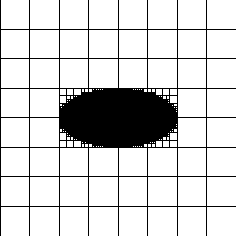
\includegraphics[width=0.32\textwidth]{./figures/integrator/gauss_1.pdf}
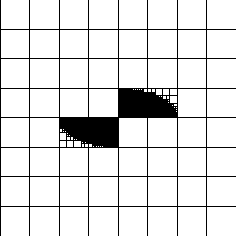
\includegraphics[width=0.32\textwidth]{./figures/integrator/gauss_2.pdf}
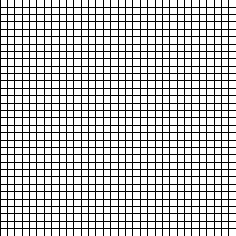
\includegraphics[width=0.32\textwidth]{./figures/integrator/gauss_3.pdf}
\end{center}
\end{figure}
\begin{footnotesize}
\begin{center}
\begin{tabular}{|c|c|c|c|c|c|c|c|c|} 
   \hline
    \textbf{Naive} & \multicolumn{2}{|c|}{Mesh 1} & \multicolumn{2}{|c|}{Mesh 2} & \multicolumn{2}{|c|}{Mesh 3}\\
    \hline
    \# of cores & Time [s] & Speedup & Time[s] & Speedup & Time [s] & Speedup \\
    \hline
    1 & 7.376 & - & 7.061 & - & 7.397 & - \\
    4 & 1.922 & \textbf{3.838} & 1.975 & \textbf{3.575} & 2.007 & \textbf{3.686} \\
    \hline
\end{tabular}
\end{center}
\begin{center}
\begin{tabular}{|c|c|c|c|c|c|c|c|c|} 
   \hline
    \textbf{3rd Gaussian}& \multicolumn{2}{|c|}{Mesh 1} & \multicolumn{2}{|c|}{Mesh 2} & \multicolumn{2}{|c|}{Mesh 3}\\
    \hline
    \# of cores & Time [s] & Speedup & Time[s] & Speedup & Time [s] & Speedup \\
    \hline
    1 & 13.873 & - & 10.410 & - & 74.364 & - \\
    4 & 3.633 & \textbf{3.819} & 3.679 & \textbf{2.830} & 19.418 & \textbf{3.830} \\
    \hline
\end{tabular}
\end{center}
\end{footnotesize}
\end{frame}

\begin{frame}\begin{footnotesize}
\begin{gather*}
 \Omega = [-2,2]^2 \quad \phi(x,y) = \max{ \left  \{ |x-0.25|-0.75, |y-0.25|-0.75 \right \} } \\
 f(x,y) = (x^2+y^2) \left[ \cos{(\pi x)} + \sin{(\pi y) }\right ]\mathbb{I}_{ \{ \phi(x,y) \leq 0 \}} \quad \int_{\Omega} f(x,y) dx dy = \frac{3(-16 - 12 \pi + 7 \pi^2)}{8 \pi^3} \simeq 0.186109
\end{gather*}\end{footnotesize}
 \begin{figure}[!h]
\begin{center}
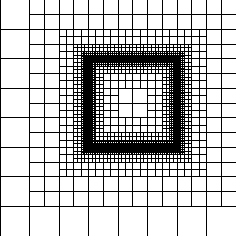
\includegraphics[width=0.32\textwidth]{./figures/integrator/square_1.pdf}
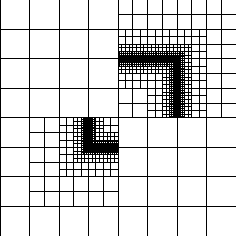
\includegraphics[width=0.32\textwidth]{./figures/integrator/square_2.pdf}
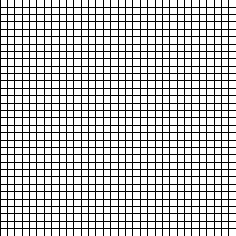
\includegraphics[width=0.32\textwidth]{./figures/integrator/square_3.pdf}
\end{center}
\end{figure}
\begin{footnotesize}
\begin{center}
\begin{tabular}{|c|c|c|c|c|c|c|c|c|} 
   \hline
    \textbf{Naive} & \multicolumn{2}{|c|}{Mesh 1} & \multicolumn{2}{|c|}{Mesh 2} & \multicolumn{2}{|c|}{Mesh 3}\\
    \hline
    \# of cores & Time [s] & Speedup & Time[s] & Speedup & Time [s] & Speedup \\
    \hline
    1 & 6.426 & - & 6.634 & - & 7.532 & - \\
    4 & 1.686 & \textbf{3.811} & 1.757 & \textbf{3.776} & 1.948 & \textbf{3.867} \\
    \hline
\end{tabular}
\end{center}
\begin{center}
\begin{tabular}{|c|c|c|c|c|c|c|c|c|} 
   \hline
    \textbf{3rd Gaussian}& \multicolumn{2}{|c|}{Mesh 1} & \multicolumn{2}{|c|}{Mesh 2} & \multicolumn{2}{|c|}{Mesh 3}\\
    \hline
    \# of cores & Time [s] & Speedup & Time[s] & Speedup & Time [s] & Speedup \\
    \hline
    1 & 7.057 & - & 6.914 & - & 75,551 & - \\
    4 & 1.902 & \textbf{3.710} & 1.987 & \textbf{3.480} & 20.245 & \textbf{3.732} \\
    \hline
\end{tabular}
\end{center}
\end{footnotesize}
\end{frame}

\begin{frame}
\begin{footnotesize}
 \begin{gather*}
  \Omega = [0,8]^2 \quad \phi(x,y) = \min_{i,j=0,\dots,3} \left ( \sqrt{(x-(2i+1))^2 + (y-(2j+1))^2}-0.15\right ) \quad f(x,y) = \mathbb{I}_{\{ \phi(x,y) \leq 0\}} \\
  \int_{\Omega} \psi(x,y) dx dy = \frac{9 \pi}{25}
 \end{gather*}
\end{footnotesize}
 \begin{figure}[!h]
\begin{center}
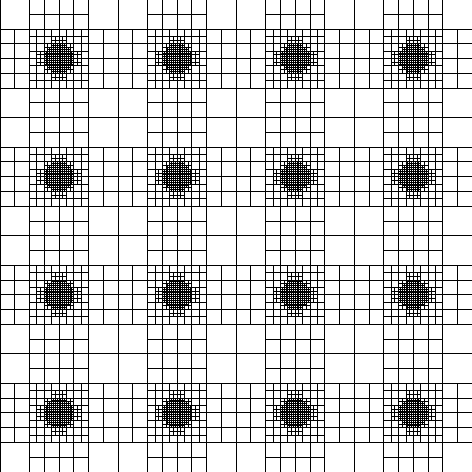
\includegraphics[width=0.32\textwidth]{./figures/integrator/unif_1.pdf}
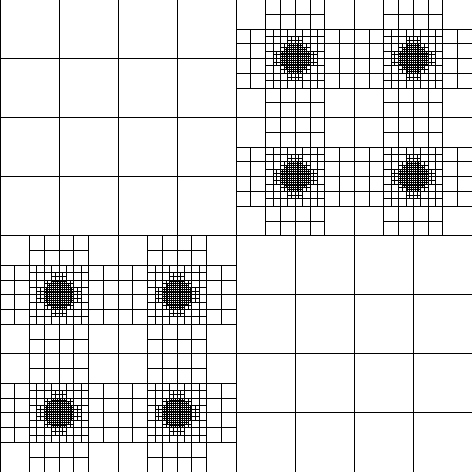
\includegraphics[width=0.32\textwidth]{./figures/integrator/unif_2.pdf}

\includegraphics[width=0.32\textwidth]{./figures/integrator/unif_3.pdf}
\end{center}
\end{figure}
\begin{footnotesize}
\begin{center}
\begin{tabular}{|c|c|c|c|c|c|c|c|c|} 
   \hline
    \textbf{Naive} & \multicolumn{2}{|c|}{Mesh 1} & \multicolumn{2}{|c|}{Mesh 2} & \multicolumn{2}{|c|}{Mesh 3}\\
    \hline
    \# of cores & Time [s] & Speedup & Time[s] & Speedup & Time [s] & Speedup \\
    \hline
    1 & 8.145 & - & 7.445 & - & 12.063 & - \\
    4 & 2.146 & \textbf{3.795} & 2.186 & \textbf{3.406} & 3.167 & \textbf{3.809} \\
    \hline
\end{tabular}
\end{center}
\begin{center}
\begin{tabular}{|c|c|c|c|c|c|c|c|c|} 
   \hline
    \textbf{3rd Gaussian}& \multicolumn{2}{|c|}{Mesh 1} & \multicolumn{2}{|c|}{Mesh 2} & \multicolumn{2}{|c|}{Mesh 3}\\
    \hline
    \# of cores & Time [s] & Speedup & Time[s] & Speedup & Time [s] & Speedup \\
    \hline
    1 & 9.165 & - & 7.956 & - & 116.295 & - \\
    4 & 2.375 & \textbf{3.859} & 2.449 & \textbf{3.249} & 30.707 & \textbf{3.787} \\
    \hline
\end{tabular}
\end{center}
\end{footnotesize}
\end{frame}

\begin{frame}
The inhomogeneity of the mesh does not play a very huge role since the time needed to construct and refine the mesh dominates over the time needed to integrate on it.
Nevertheless, where the inhomogeneity is really strong, we observe the most important differences.
\end{frame}


\subsection{Image compression}
\begin{frame}
Three different $\epsilon$: $\epsilon = 0.012, 0.024, 0.048$.
\begin{center}
 \begin{figure}[!h]
 \begin{footnotesize}
  Original figures size: 262144 px. 
 \end{footnotesize}\\
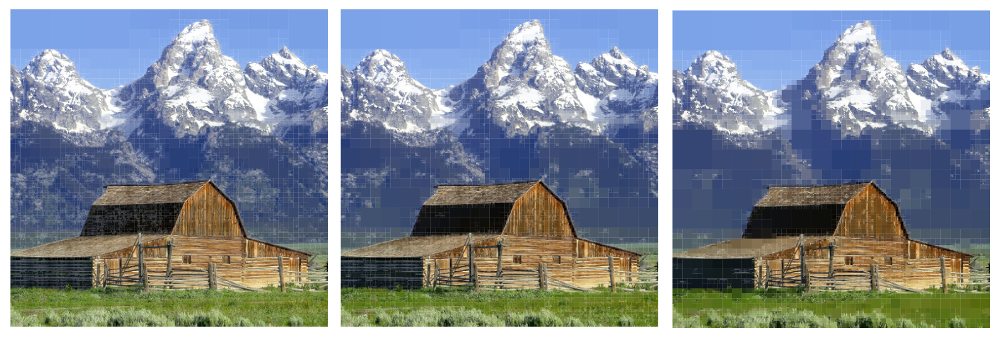
\includegraphics[width=0.9\textwidth]{./figures/s1_comp_small} \\
\begin{footnotesize}131509 px - comp. ratio = 1.99 \hfill 84808 px - comp. ratio = 3.09 \hfill 38152 px - comp. ratio = 6.87 \end{footnotesize} \\
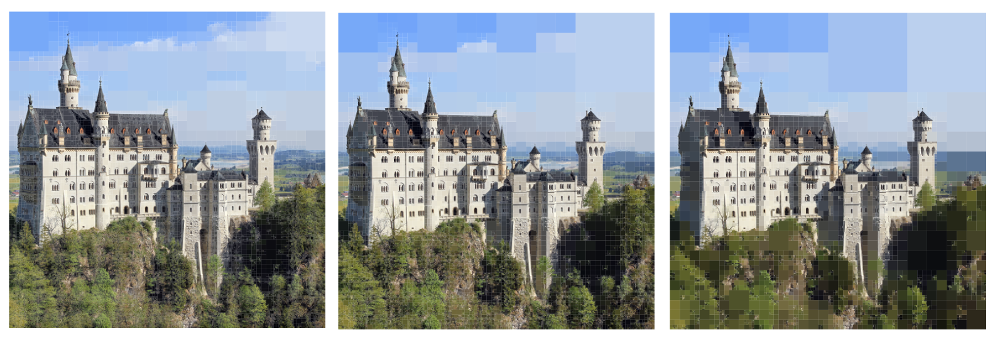
\includegraphics[width=0.9\textwidth]{./figures/s2_comp_small}\\
\begin{footnotesize}115438 px - comp. ratio = 2.27 \hfill 69259 px - comp. ratio = 3.78 \hfill 27394 px - comp. ratio = 9.57 \end{footnotesize} \\
\end{figure}
\end{center}
\end{frame}

\begin{frame}
\begin{center}
 \begin{figure}[!h]
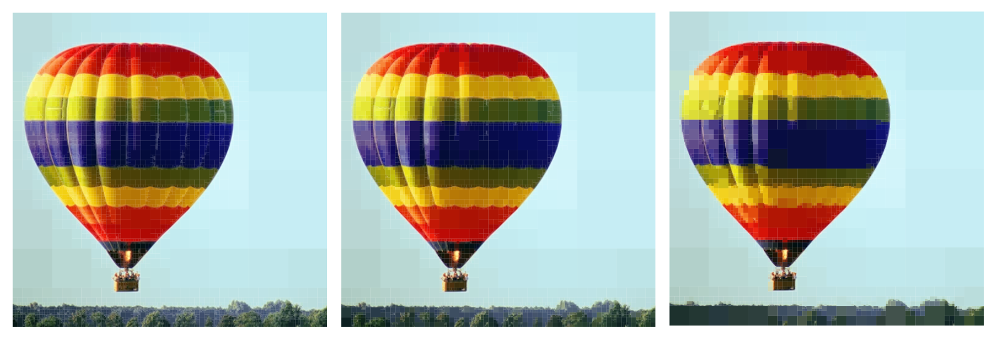
\includegraphics[width=0.9\textwidth]{./figures/s3_comp_small} \\
\begin{footnotesize}32188 px - comp. ratio = 8.14 \hfill 16405 px - comp. ratio = 15.98 \hfill 6571 px - comp. ratio = 39.89 \end{footnotesize} \\
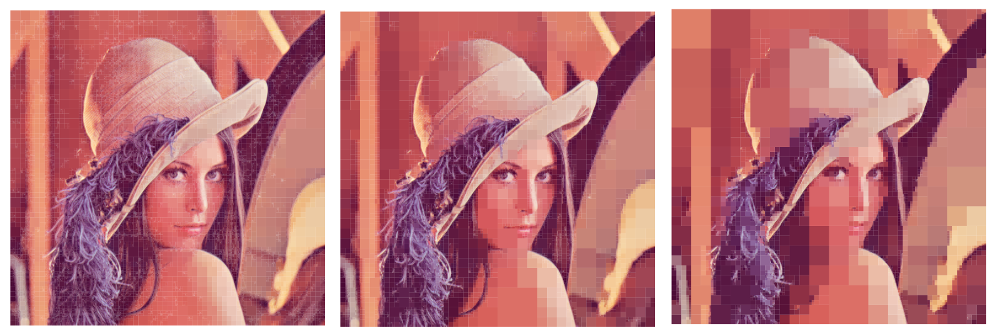
\includegraphics[width=0.9\textwidth]{./figures/s4_comp_small}\\
\begin{footnotesize}75172 px - comp. ratio = 3.49 \hfill 29890 px - comp. ratio = 8.77 \hfill 8902 px - comp. ratio = 29.45 \end{footnotesize} \\
\end{figure}
\end{center}
\end{frame}

\begin{frame}
\begin{center}
 \begin{figure}[!h]
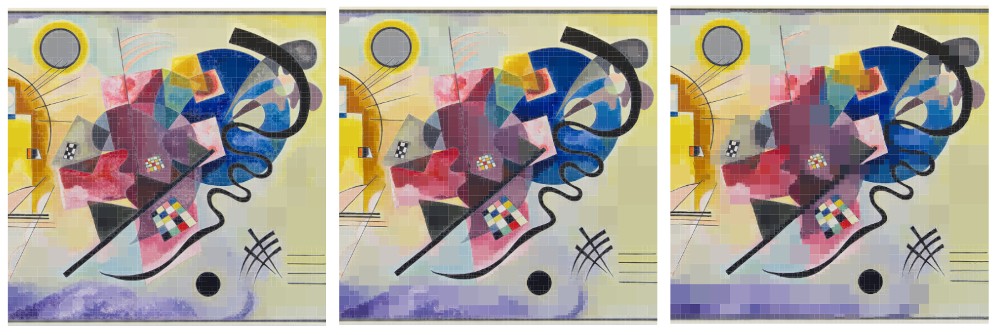
\includegraphics[width=0.9\textwidth]{./figures/s6_comp_small}\\
\begin{footnotesize}171517 px - comp. ratio = 1.53 \hfill 85258 px - comp. ratio = 3.07 \hfill 24466 px - comp. ratio = 10.71
\end{footnotesize} \\
\end{figure}
\end{center}
\end{frame}

\section{Conclusions and perspectives}

\begin{frame}
 \begin{itemize}
  \item Different way of storing the tree: time-efficiency, memory-efficiency, possibility of recovering neighbors.
  \item Implement a way of finding neighbors (in our implementation, every cell should store a pointer to its father).
  \item Improve data distribution between cores.
 \end{itemize}

\end{frame}


\section{Bibliography}

\end{document}
